\documentclass[10pt,landscape]{article}
\usepackage{amssymb,amsmath,amsthm,amsfonts}
\usepackage{multicol,multirow}
\usepackage{calc}
\usepackage{ifthen}
\usepackage[landscape]{geometry}
\usepackage[colorlinks=true,citecolor=blue,linkcolor=blue]{hyperref}

\usepackage{titlesec}
\titleformat*{\paragraph}{\itshape}


\ifthenelse{\lengthtest { \paperwidth = 11in}}
    { \geometry{top=.5in,left=.5in,right=.5in,bottom=.5in} }
	{\ifthenelse{ \lengthtest{ \paperwidth = 297mm}}
		{\geometry{top=1cm,left=1cm,right=1cm,bottom=1cm} }
		{\geometry{top=1cm,left=1cm,right=1cm,bottom=1cm} }
	}
\pagestyle{empty}
\makeatletter
\renewcommand{\section}{\@startsection{section}{1}{0mm}%
                                {-1ex plus -.5ex minus -.2ex}%
                                {0.5ex plus .2ex}%x
                                {\normalfont\large\itshape}}
\renewcommand{\subsection}{\@startsection{subsection}{2}{0mm}%
                                {-1explus -.5ex minus -.2ex}%
                                {0.5ex plus .2ex}%
                                {\normalfont\normalsize\itshape}}
\renewcommand{\subsubsection}{\@startsection{subsubsection}{3}{0mm}%
                                {-1ex plus -.5ex minus -.2ex}%
                                {1ex plus .2ex}%
                                {\normalfont\small\itshape}}
\makeatother
\setcounter{secnumdepth}{0}
\setlength{\parindent}{0pt}
\setlength{\parskip}{0pt plus 0.5ex}
% -----------------------------------------------------------------------

\title{String Sheet}

\newcommand*{\EndZeichen}{\texttt{\$}}
\usepackage{mathtools} % coloneqq

\newcommand{\IC}{\mathbin{{.}\,{.}}} %interval '\IC{}'

\newcommand*{\abs}[1]{\ensuremath{|#1|}} % | |
\newcommand*{\menge}[1]{\ensuremath{\{#1\}}} % | |

\newcommand*{\instancename}[1]{\ensuremath{\mathsf{#1}}} %for instance names
\newcommand*{\LPF} {\instancename{LPF}}
\newcommand*{\LCPA} {\instancename{LCP}}
\newcommand*{\PLCP}{\instancename{PLCP}}
\newcommand*{\ISA} {\instancename{ISA}}
\newcommand*{\SA}  {\instancename{SA}}
\newcommand*{\BWT}  {\instancename{BWT}}
\newcommand*{\arrC}  {\instancename{C}}

\newcommand*{\textT}  {\ensuremath{T}}
\newcommand*{\textS}  {\ensuremath{S}}

\newcommand*{\ibeg}[1]{\mathsf{b}(#1)}% beginning position of the interval #1
\newcommand*{\iend}[1]{\mathsf{e}(#1)}% ending position of the interval #1

\newcommand*{\functionname}[1]{{\ensuremath{\renewcommand{\rmdefault}{ptm}\fontfamily{ppl}\selectfont\textrm{\textup{#1}}}}} %for instance names
\newcommand*{\select}{\functionname{select}}
\newcommand*{\rank}{\functionname{rank}}
\newcommand*{\lcp}{\functionname{lcp}}


\newcommand*{\argmax}{\operatorname{argmax}}
\newcommand*{\argmin}{\operatorname{argmin}}

\usepackage{tikz}
\usetikzlibrary{matrix,fit}

\usepackage{lilyglyphs}

% -----------------------------------------------------------------------
\begin{document}

\raggedright
\footnotesize

\begin{center}
     \Large{\textbf{String Sheet \twoBeamedQuavers}} \\
\end{center}
\begin{multicols}{2}
\setlength{\premulticols}{1pt}
\setlength{\postmulticols}{1pt}
\setlength{\multicolsep}{1pt}
\setlength{\columnsep}{2pt}


\section{Defs}
\begin{multicols}{2}
\begin{itemize}
\item $\prec \coloneqq$ lexicographic order
	\item $\varepsilon \coloneqq$  empty string
	\item $\textT \coloneqq$ string, $T[\abs{T}] \coloneqq \EndZeichen$
	\item $\textS \lhd \textT :\Leftrightarrow \textS[\lcp(\textS,\textT)] < \textT[\lcp(\textS,\textT)]$
	\item $\textS \prec \textT :\Leftrightarrow  \textS \lhd \textT \vee \textS$ is proper prefix of $\textT$
\end{itemize}
\end{multicols}

\section{Trees}

\begin{multicols}{2}
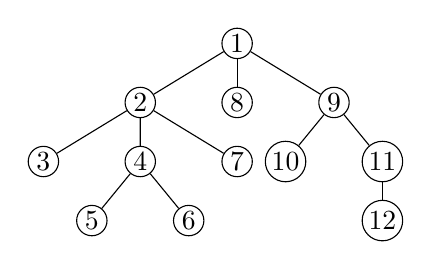
\begin{tikzpicture}[every node/.style={shape=circle,draw,inner sep=0.1em},scale=0.5, sibling distance=7em]
\node {1}
	child {node {2} 
		child {node {3}}
		child {node {4}
			child {node {5}}
			child {node {6}}
			}
		child {node {7}}
		}
	child {node {8} }
	child {node {9}
		child {node {10}}
		child {node {11}
			child {node {12}}
			}
		}
	;
\end{tikzpicture}
\begin{itemize}
	\item   DFUDS~\cite{benoit05dfuds}
	\item   LOUDS~\cite{jacobson89rank}
	\item   BP~\cite{jacobson89rank}
\end{itemize}
   
\end{multicols}

\tikzstyle{mymatrix} = [matrix of nodes,nodes in empty cells
,row sep=0
,inner sep=0.4em
,row 1/.style={nodes={font=\tiny,inner sep=0}}
,row 3/.style={nodes={font=\scriptsize,inner sep=0}}
,row 4/.style={nodes={font=\scriptsize}}
,column 1/.style={nodes={text width=3.5em}}
]

\begin{tikzpicture}
\matrix (DFUDS) [mymatrix]
{%
   & 1& 2& 3&4& 5& 6&7& 8&9&10&11&12&13&14&15&16&17&18&19&20&21&22&23&24\\
DFUDS & ( & ( & ( & ( & ) & ( & ( & ( & ) & ) & ( & ( & ) & ) & ) & ) & ) & ( & ( & ) & )  & (  & ) & )   \\
id    &   &   &   &   &   &   &   &   &   &   &   &   &   &   &   &   &   &   &   &   &    &    &   &     \\
};
\newcommand*{\DrawId}[3]{%
\node[fit=(DFUDS-3-#1)(DFUDS-3-#2),font=\scriptsize]{#3};
\begin{scope}[transform canvas={yshift=-0.1em}]
\draw (DFUDS-2-#1.south |- DFUDS-2-1.south) -- (DFUDS-2-#2.south |- DFUDS-2-1.south);
\end{scope}
}
\DrawId{3}{6}{1}
\DrawId{7}{10}{2}
\DrawId{11}{11}{3};
\DrawId{12}{14}{4};
\DrawId{15}{15}{5};
\DrawId{16}{16}{6};
\DrawId{17}{17}{7};
\DrawId{18}{18}{8};
\DrawId{19}{21}{9};
\DrawId{22}{22}{10};
\DrawId{23}{24}{11};
\DrawId{25}{25}{12};
\end{tikzpicture}


\begin{tikzpicture}
\matrix (LOUDS) [mymatrix]
{%
      & 1 & 2 & 3 & 4 & 5 & 6 & 7 & 8 & 9 & 10 & 11 & 12 & 13 & 14 & 15 & 16 & 17 & 18 & 19 & 20 & 21 & 22 & 23 & 24 & 25\\
LOUDS & ( & ) & ( & ( & ( & ) & ( & ( & ( & )  & )  & (  & (  & )  & )  & (  & (  & )  & )  & )  & (  & )  & )  & )  & ) \\
id    & 1 &   & 2 & 8 & 9 &   & 3 & 4 & 7 &    &    &10  &11  &    &    & 5  & 6  &    &    &    & 12 &    &    & & \\
parent     &   &   &   &   &   &   &   &   &   &    &    &    &    &    &    &    &    &    &    &    &    &    &    & & \\
};

\newcommand*{\DrawParent}[3]{%
\node[fit=(LOUDS-4-#1)(LOUDS-4-#2),font=\scriptsize]{#3};
\begin{scope}[transform canvas={yshift=-0.1em}]
\draw (LOUDS-3-#1.south |- LOUDS-3-1.south) -- (LOUDS-3-#2.south |- LOUDS-3-1.south);
\end{scope}
}

\DrawParent{4}{7}{1}
\DrawParent{8}{11}{2}
\DrawParent{12}{12}{8}
\DrawParent{13}{15}{9}
\DrawParent{16}{16}{3}
\DrawParent{17}{19}{4}
\DrawParent{20}{20}{7}
\DrawParent{21}{21}{10}
\DrawParent{22}{23}{11}
\DrawParent{24}{24}{5}
\DrawParent{25}{25}{6}
\DrawParent{26}{26}{12}
\end{tikzpicture}



\begin{tikzpicture}
\matrix (BP) [mymatrix]
{%
   & 1& 2& 3&4& 5& 6&7& 8&9&10&11&12&13&14&15&16&17&18&19&20&21&22&23&24\\
BP & (& (& (&)& (& (&)& (&)& )& (&)& )& (&)& (& (&)&  (& (&)& )&  )& ) \\
   &  &  &  & &  &  & &  & &  &  & &  &  & &  &  & &   &  & &  &   &   \\
};
\newcommand*{\DrawId}[4]{%
\draw (BP-2-#1.south |- BP-2-1.south)  |- node [midway,anchor=north] {#3} ([yshift=-#4]BP-2-#2.south) -- (BP-2-#2.south |- BP-2-1.south);
}
\DrawId{4}{5}{3}{0.5em}

\DrawId{6}{11}{4}{2em}
\DrawId{7}{8}{5}{0.5em}
\DrawId{9}{10}{6}{0.5em}
\DrawId{12}{13}{7}{0.5em}
\DrawId{3}{14}{2}{3.5em}
\DrawId{15}{16}{8}{0.5em}
\DrawId{18}{19}{10}{0.5em}
\DrawId{21}{22}{12}{0.5em}
\DrawId{20}{23}{11}{2em}
\DrawId{17}{24}{9}{3.5em}
\DrawId{2}{25}{1}{5em}
\end{tikzpicture}



\section{Arrays}



\begin{itemize}
	\item $\SA$: $\textT[\SA[i-1]\IC{}n] \prec \textT[\SA[i]\IC{}n]~\forall i \in [2\IC{}n]$~\cite{manber93sa}
	\item $\LCPA[i] = \lcp(\SA[i-1], \SA[i])~\forall i \in [2\IC{}n]$
	\item $\PLCP[ {\SA[i]} ] \coloneqq \LCPA[i]$~\cite{kasai01lcp}
	\item $\LPF[j] \coloneqq \max\{\ell \mid \exists i \in [1\IC{}j-1] : \textT[i\IC{}i+\ell-1] = \textT[j\IC{}j+\ell-1]\}$~\cite{franek03lpf,crochemore08lpf}
\end{itemize}
backward
\begin{itemize}
	\item $\BWT[i] \coloneqq \textT[\SA[i]-1]~\forall i \not= \ISA[1]$, $\BWT[\ISA[1]] \coloneqq \textT[n] = \EndZeichen$~\cite{burrows94bwt}
	\item $\Phi[i] \coloneqq \SA[ {\ISA[i]} - 1]~\forall i \not= \ISA[1]$, $\Phi[\ISA[1]] \coloneqq n$~\cite{karkkainen09plcp}
	\item $\Phi^{k}[i] = \SA[ ({\ISA[i]} + n - k-1 \mod n) + 1]~\forall i,k \in [1\IC{}n]$.
\end{itemize}
forward
\begin{itemize}
	\item $\Psi[i] \coloneqq \ISA[ {\SA[i]} + 1 ]~\forall i \not= \ISA[n]$, $\Psi[\ISA[n]] \coloneqq \ISA[1]$
	\item $\Psi^{k}[i] = \SA[ ({\ISA[i]} + k-1 \mod n) + 1]~\forall i,k \in [1\IC{}n]$.
\end{itemize}

irreducible
\begin{itemize}
	\item $\LCPA[i] = \PLCP[\SA[i]]$ irreducible $:\Leftrightarrow$ $\BWT[i] = \BWT[i-1]$.
	\item $\PLCP[i]$ irreducible $\Rightarrow \PLCP[i] = \PLCP[i-1] - 1 \wedge \Phi[i] = \Phi[i-1]+1$. \cite{karkkainen09plcp}
\end{itemize}



\section{Periods}

Periodicity Lemma~\cite{fine65uniqueness}:
$\textT$ has periods~$p$ and~$p'$ with $p+p' \le \abs{\textT} \Rightarrow \gcd(p,p')$ is period of~$\textT$.


\section{Lyndon}

$\textT$ Lyndon $:\Leftrightarrow \textT \lhd \textT[i\IC{}] \forall i \in [2\IC{}\abs{\textT}]$

If $\textT$ Lyndon, then
\begin{multicols}{2}
\begin{itemize}
	\item $\nexists$ period of $\textT$
	\item $\textT$ is border-free
	\item $\textT \prec \textS \wedge \textS$ Lyndon $\Rightarrow \textT \prec \textT\textS \prec \textS \Rightarrow \textT \textS$ Lyndon \cite{chen58lyndon}
\end{itemize}
\end{multicols}

\section{Factorization}
Let $\textT = F_1 \cdots F_z$.

\paragraph{Lyndon factorization}
	\begin{itemize}
	\item $F_i$ Lyndon  $\forall i \in [1\IC{}z] \wedge F_i \succeq F_{i+1}~\forall i\in[1\IC{}z)$  \cite{chen58lyndon}
		\item $F_i = \textT[\ibeg{F_i} \IC{} x]$ where $x \coloneqq \argmin_{j > \ibeg{F_i}} \ISA[j] > \ISA[\ibeg{F_i}]$
		\item $F_i$ longest Lyndon prefix of $\textT[\ibeg{F_i}\IC{}]$
	\end{itemize}


\newcommand*{\SubStrPrev}[2]{\mathcal{S}_{#1}(#2)}


\paragraph{Classic LZ77-factorization}
$F_x$ is the shortest prefix of $F_x \cdots F_z$ occurring exactly once in $F_1 \cdots F_x$~\cite{ziv77lz}.

\paragraph{LZ78 factorization}
$F_x=F'_x c$ with $F'_x = \argmax_{S \in \menge{F_y \mid y < x} \cup \menge{\varepsilon} } \abs{S}$ and $c\in\Sigma$, $\forall x \in [1\IC{} z]$~\cite{ziv78lz}.

\paragraph{$s$-factorization}
$F_x \coloneqq \argmax_{S \in \SubStrPrev{j}{T} \cup \Sigma} \abs{S}~\forall x \in [1\IC{} z]$, where $j \coloneqq \abs{F_1\cdots F_{x-1}}+1$
and $\SubStrPrev{j}{\textT}$ is the set of substrings of $\textT$ starting \emph{strictly} before~$j$~\cite{storer82lzss}.

\paragraph{Non-overlapping $s$-factorization}
$F_x \coloneqq \argmax \menge{ \abs{S} \mid S \in \Sigma^* \text{~occurs in~} T[1\IC{}j] \text{~or~} S \in \Sigma}~\forall
x \in [1\IC{}z]$, where $j \coloneqq \abs{F_1\cdots F_{x-1}}$.


\subsection{BWT Related}

FM-index~\cite{ferragina00fmindex} backward search:
\begin{itemize}
	\item   $P:$ pattern
	\item   $\arrC[i] := \abs{\menge{j \in [1\IC{}n] : \textT[j] < i}}$
	\item   $R_i$: range of the pattern $P[i\IC{}n]$, i.e., $\textT[\SA[j]\IC{}\SA[j]+i-1] = P[i\IC{}n] \Leftrightarrow j \in R_i$
	\item $\ibeg{R_i} = \arrC[P[i]] + \rank(\ibeg{R_{i+1}} + 1, P[i])$
	\item $\iend{R_i} = \arrC[P[i]] + \rank(\iend{R_{i+1}}, P[i])$
\end{itemize}



\end{multicols}

\newpage

\begin{multicols}{3}
\bibliographystyle{abbrv}
\bibliography{literature}
\end{multicols}

\end{document}
